\chapter{Discussion and conclusions}
In this project we implemented a system for analyzing white matter architecture from DTI images.  The multithreaded implementation of the system allows parallel sampling of fiber tracts, reducing computation time on multi-processor systems.  To facilitate the algorithm's use in clinical studies, an easy to use graphical interface was created for the 3D Slicer visualization program. Furthermore, we demonstrate the system's characteristics through an analysis of fibers originating from the right internal capsule.  In this section, we will discuss some possible extensions to the system and present an outline for a potential clinical study which investigates frontal lobe fibers in schizophrenia using the stochastic tractography system developed in this thesis.

\section{Potential Extensions}
The design of the stochastic tractography system is not tightly coupled and thus allows the tensor parameter estimation engine to be replaced.  In the presented work, the stochastic tractography system estimates the log tensor model parameters through weighted least squares estimation.  More robust techniques of tensor model parameter estimation have been proposed by Koay et al. \cite{koay06}.  We can refine the fiber orientation likelihood function in our system using these improved tensor model parameter estimates.  Ideally, the DTI image and estimated B0 image should be calculated before the stochastic tractography system is run.  The stochastic tractography system can take this DTI image and B0 image as input in lieu of the DWI image.  This approach allows the researcher to use any arbitrary tensor model parameter estimation engine and additionally makes stochastic tractography faster as the tensor parameters would not need to be calculated at run time.  The modifications required to implement this feature is relatively minor, but the user interface must be designed thoughtfully to minimize the added complexity of these new options.

%Discuss finding a better prior
Although DTI images can be illumination of changes in anisotropy, DTI data alone is insufficient to determine the causes of changes in anisotropy.  Reduced anisotropy can stem from a decoherence in a fiber bundle's structure, losses in myelin, and other abnormalities.  Kubicki et al. \cite{kubickiNI05} attempted to clarify the cause of changes in anisotropy by comparing information about nerve fiber integrity that are inferred from DTI and MTR.  MTR is an MR scanning technique that provides information regarding the distribution of myelin in the brain. Anisotropy changes that are detectable by both MTR and DTI suggest alterations to the myelin.  Changes that are detectable only by DTI suggest decoherence in the fiber's structure.  The algorithm can be further extended by incorporating information from MTR measurements \cite{kubickiNI05} into the Bayesian framework.

\section{Study of frontal lobe fibers in schizophrenia}
We conclude by describing a potential group study of frontal lobe fiber differences in Schizophrenia using the stochastic tractography system.  This group study is an extension of the single subject analysis of frontal lobe fibers presented in the previous chapter.  The study also provides an opportunity to compare findings using stochastic tractography with those previously obtained from streamlining tractography on identical data sets.

%make this into a good paper
\subsection{Background}
Schizophrenia is neurological disorder whose characteristic symptoms include hallucinations and disorganized thinking.  Scientists have suggested that the pathology of schizophrenia may involve anatomical abnormalities including abnormal white matter architecture.  Clinical DTI studies have demonstrated differences in diffusion anisotropy within fiber tracts in Schizophrenia patients compared with healthy patients \cite{kubickiBiologPsych03},\cite{kubickiNI05}.

White matter architecture abnormalities related to schizophrenia may include a reduction in the integrity or amount of the myelin, increased disorganization of fibers which constitute certain fiber bundles, or a reduction in the number of fibers comprising a fiber bundle. Myelin, the fatty insulator which surrounds the axons, is believed to be a major barrier to water diffusion.  Degradation of the myelin permits increased diffusion perpendicular to the orientation of the fibers which can be observed as reduced anisotropy in DTI data.  Also the orientation of axon fibers which comprise a fiber bundle may be less directionally coherent in Schizophrenia.  Since many fibers pass through a single voxel and the resultant diffusion distribution is an average of diffusion of all water molecules in that voxel, a voxel containing fibers which are less coherent may have reduced anisotropy.  The fiber bundles may also be less dense in Schizophrenia.  A reduction in axon density would result in reduced anisotropy since water molecules are more free to diffuse perpendicularly to the tracts.  These structural deficiencies result in poorer conduction of action potentials between different regions of the brain leading to reduced functional connectivity.
\begin{figure}
  \center
  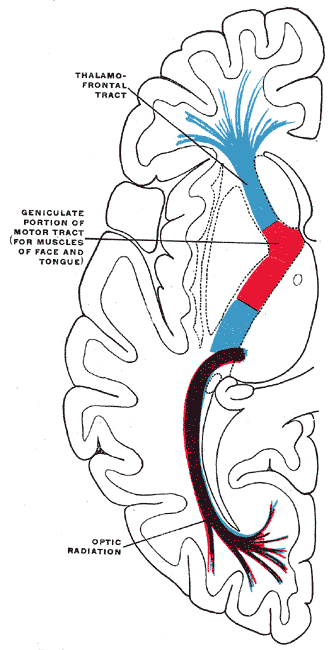
\includegraphics[height=0.5\linewidth]{frontalcortexfibers}
	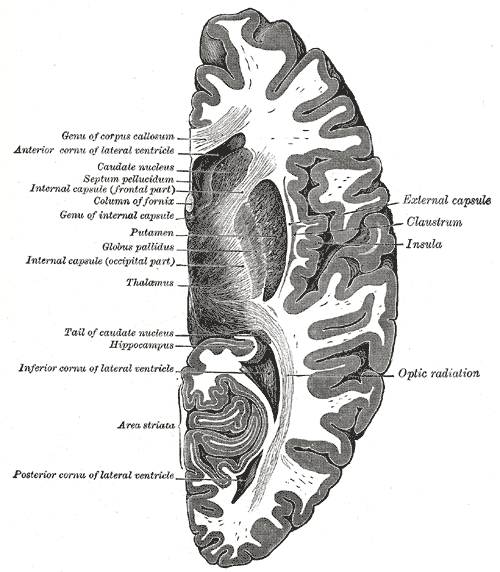
\includegraphics[height=0.5\linewidth]{thalamus}
	\caption{The Thalamus, the Internal Capsule and fibers.  We wish to characterize the fibers which originate in the thalamus, pass through the internal capsule and end in the frontal cortex.  This image is from Gray's Anatomy.}
	\label{fig:frontallobefibers}
\end{figure}
The fibers that connect the thalamus and the frontal lobe are believed to be involved in memory formation.  These fibers are depicted in figure \ref{fig:frontallobefibers}.  Since Schizophrenia patients have difficulty forming and organizing memory, deficiencies in these fibers may explain these symptoms.  Additionally these fibers present an interesting tractography problem because there are many other fibers which cross this set of fibers on their way to the frontal cortex.  In these regions of crossing, the diffusion is averaged with the crossing fibers resulting in a diffusion profile with reduced anisotropy.  This is precisely the situation that stochastic tractography can be useful since streamlining methods would terminate in regions of low anisotropy possibly never reaching the frontal cortex.  In this future study, we will analyze these fibers in schizophrenia and control groups to determine whether schizophrenia patients exhibit lower tract-averaged fractional anisotropy than the control group.  Additionally, we will compare results obtained using stochastic tractography with previous streamline tractography results.

%show where the labels are using picture
\subsection{Method}
We will first obtain DWI data sets for as many schizophrenia and control subjects as possible.  Each DWI data set will consist of at least six gradient weighted images and one baseline image as this is the minimum required for the stochastic tractography system.  Additionally we will create a white matter map for each subject either by a segmentation of an additional anatomical image obtained during the DWI acquisition or through the segmentation of the B0 image.  Label maps for the right and left internal capsules for each subject are created through expert manual segmentation.  An additional ROI is placed in the frontal lobe to isolate fibers which originate in the internal capsules and proceed towards the frontal lobe.

The stochastic tractography system will then used to generate tract length and tract-averaged FA statistics for tracts which originate in the right internal capsule and pass through the frontal lobe ROI.  The system will be run again for tracts which originate in the left internal capsule and pass through frontal lobe ROI.  These analysis will be performed for all subjects.  Tracts will be sampled until the mean of the length and tract-averaged FA distributions show a degree of stability with respect to the number of samples.

Assuming that the mean tract-averaged FA is normally distributed, a t-test can be used to determine whether the mean of the mean tract-averaged FA differs significantly between schizophrenia subjects and normal subjects.  The same is performed for the distribution of tract lengths.

Finally, these results will be compared with the results of a streamline tractography based study on the same data set by Rosenberger\cite{Rosenberger07}.  This study found significant differences in the mean of the mean tract-averaged FA between schizophrenia and control groups.

\section{Summary}
The field of neuroscience has made great advances in recent years.  Further understanding of how the brain functions and the diseases which affect it will depend on our ability to study white matter architecture.  In-vivo observation techniques such as Diffusion Tensor MRI play a crucial role in the study of white matter architecture.  As observation methods become more sophisticated, our tools for inference must also be sufficiently sophisticated to extract the valuable information hidden in these observations.  The stochastic tractography system we have presented in this thesis provide neuroscientists with an efficient and easy to use tool to characterize white matter architecture.

%Refine the algorithm
%	-currently the algorithm terminates when the generated fiber encounters a region of %anisotropy below some set value
%		-in reality, fibers may exist that pass through areas of low anisotropy
%		-this is possible in regions with many crossing fibers
%			-perhaps it would be possible to terminate instead on the overall magnitude of %diffusion.  If total diffusion is above/below a certain threshold than end diffusion.

%Once this data has been obtained the connectivity map will be generated for all subjects.  The connectivity maps will be compared to determine whether there are differences in the connectivity distributions of the regions that were determined by Kubicki et al. to differ either under DTI or MTR measurements, between the patients and the control groups.  The regions that differed under fractional anisotropy (FA), a summary measure of DTI, include the fornix, the corpus callosum, the  cingulum bundle, the superior occipito-frontal fasciculus, the internal capsule, the right inferior occipito-frontal fasciculus and the left arcuate fasciculus.  The regions that differed under MTR were the corpus callosum, fornix, right internal capsule, superior occipito-frontal fasciculus and the right posterior cingulum bundle.
